\section{General concepts using 1D DC resistivity inversion}\label{sec:dc1d}
{\em See cpp/py files in the directory \file{doc/tutorial/code/dc1d}.}
\subsection{Smooth inversion}\label{sec:dc1dsmooth}
{\em Example file \file{dc1dsmooth.cpp}.}\\
Included into the GIMLi library are several electromagnetic 1d forward operators.
For direct current resistivity there is a semi-analytical solution using infinite sums that are approximated by Ghosh filters. 
The resulting function calculates the apparent resistivity of any array for a given resistivity and thickness vector.
There are two main parameterisation types:
\begin{itemize}
	\item a fixed parameterisation where only the parameters are varied 
	\item a variable parameterisation where parameters and geometry is varied
\end{itemize}

Although for 1d problems the latter is the typical one (resistivity and thickness), we start with the first since it is more general for 2d/3d problems and actually easier.
Accordingly, in the file dc1dmodelling.h/cpp two classes called \cw{DC1dRhoModelling} and \cw{DC1dBlockModelling} are defined.
For the first we first define a thickness vector and create a mesh using the function \cw{createMesh1d}.
The the forward operator is initialized with the data.

\begin{lstlisting}[language=C++]
    RMatrix abmnr; loadMatrixCol( abmnr, dataFile ); //! read data
    RVector ab2 = abmnr[0], mn2 = abmnr[1], rhoa = abmnr[2]; //! 3 columns
    RVector thk( nlay-1, max(ab2) / 2 / ( nlay - 1 ) ); //! const. thickn.
    DC1dRhoModelling f( thk, ab2, mn2 ); //! initialise forward operator
\end{lstlisting}

Note that the mesh generation can also be done automatically using another constructor.
However most applications will read or create a mesh from in application and pass it.

By default, the transformations for data and model are identity transformations.
We initialise two logarithmic transformations for the resistivity and the apparent resistivity by 
\begin{lstlisting}[language=C++]
    RTransLog transRho;
    RTransLog transRhoa;
\end{lstlisting}

Alternatively, we could set lower/upper bounds for the resistivity using
\begin{lstlisting}[language=C++]
    RTransLogLU transRho( lowerbound, upperbound);
\end{lstlisting}
Appendix \ref{app:trans} gives an overview on available transformation functions.

Next, the inversion is initialized and a few options are set
\begin{lstlisting}[language=C++]
    RInversion inv( data.rhoa(), f, verbose );
    inv.setTransData( transRhoa );           //! data transform
    inv.setTransModel( transRho );           //! model transform
    inv.setRelativeError( errPerc / 100.0 ); //! constant relative error
\end{lstlisting}

A starting model of constant values (median apparent resistivity) is defined
\begin{lstlisting}[language=C++]
    RVector model( nlay, median( data.rhoa() ) ); //! constant vector
    inv.setModel( model );                        //! starting model
\end{lstlisting}

Finally, the inversion is called and the model is retrieved using \lstinline|model = inv.run();|

A very important parameter is the regularisation parameter $\lambda$ that controls the strength of the smoothness constraints (which are the default constraint for any 1d/2d/3d mesh).
Whereas $w^c$ and $w^m$ are dimensionless and 1 by default, $\lambda$ has, after eq. (\ref{eq:min}), the reciprocal and squared unit of $m$ and can thus have completely different values for different problems\footnote{The regularisation parameter has therefore to be treated logarithmically.}.
However, since often the logarithmic transform is used, the default value of $\lambda=20$ is often a first guess.
Other values are set by
\begin{lstlisting}
    inv.setLambda( lambda ); //! set regularisation parameter
\end{lstlisting}

In order to optimise $\lambda$, the L-curve \citep{guentherruecker06,guentherdiss} can be applied to find a trade-off between data fit and model roughness by setting \lstinline|inv.setOptimizeLambda(true);|.
For synthetic data or field data with well-known errors we can also call \lstinline|model = inv.runChi1();|, which varies $\lambda$ from the starting value such that the data are fitted within noise ($\chi^2=1$).
We created a synthetic model with resistivities of 100(soil)-500(unsaturated)-20(saturated)-1000(bedrock) $\Omega$m and thicknesses of 0.5, 3.5 and 6 meters.
A Schlumberger sounding with AB/2 spacings from 1.0 to 100\,m was simulated and 3\% noise were added.
Data format of the file \file{sond1-100.dat} is the unified data format\footnote{See \url{www.resistivity.net?unidata} for a description.}.

\begin{figure}[htbp]
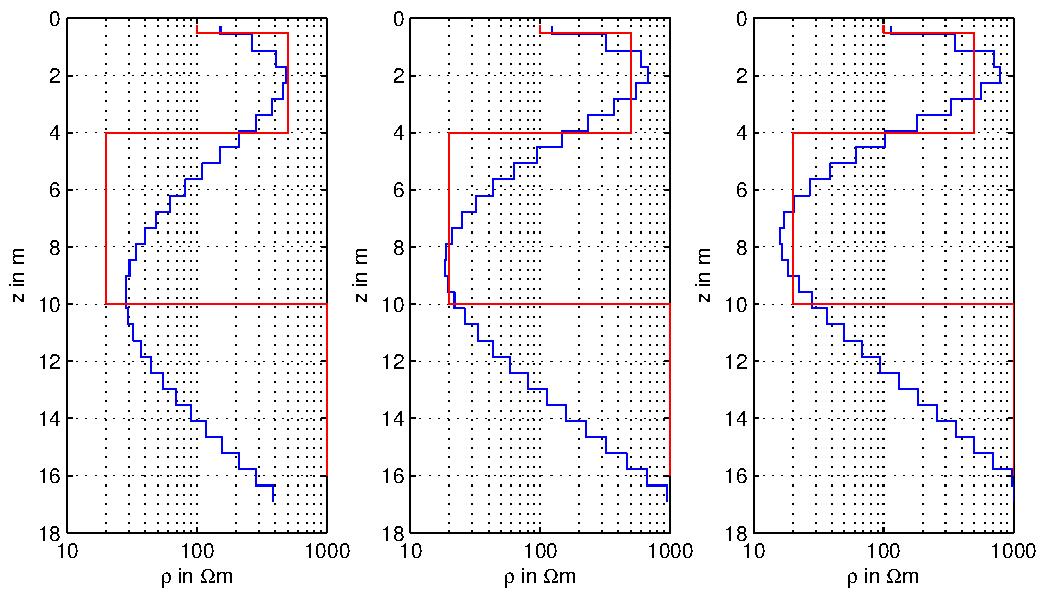
\includegraphics[width=\textwidth]{sond1-100-3lambdas}\\[-3ex]
~~~a\hfill ~~~b \hfill ~~~c \hfill ~
\caption{Smooth 1d resistivity inversion results for a) $\lambda=200\Rightarrow \chi^2=11.1$/rrms=10.1\%, b) $\lambda=20\Rightarrow \chi^2=1.2$/rrms=3.3\%, and c) $\lambda=2\Rightarrow \chi^2=0.6$/rrms=2.4\%, red-synthetic model, blue-estimated model}\label{fig:dc1d-3lambda}
\end{figure}

Figure~\ref{fig:dc1d-3lambda} shows the inversion result for the three different regularisation parameters 300, 30 and 3.
Whereas the first is over-smoothed, the other are much closer at the reality.
The rightmost figure over-fits the data ($\chi^2=0.3<1$) but is still acceptable.
The L-curve method yields a value of $\lambda=2.7$, which is too low.
However, if we apply the $\chi^2$-optimization we obtain a value of $\lambda=15.2$ and with it the data are neither over- nor under-fitted.

%%%%%%%%%%%%%%%%%%%%%%%%%%%%%%%%%%%%%%%%%%%%%%%%%%%%%%%%%%%%%%%%%%%%%%%%%%%
\subsection{Block inversion}\label{sec:dc1dblock}
{\em Example file \file{dc1dblock.cpp} in the directory \file{doc/tutorial/code/dc1d}.}\\
Alternatively, we might invert for a block model with unknown layer thickness and resistivity.
We change the mesh generation accordingly and use the forward operator \lstinline|DC1dModelling|:
\begin{lstlisting}[language=C++]
    DC1dModelling f( nlay, ab2, mn2 );
\end{lstlisting}

\lstinline|createMesh1DBlock| creates a block model with two regions\footnote{With a second argument \lstinline|createMesh1DBlock| can create a block model with thickness and several parameters for a multi-parameter block inversion.}.
Region 0 contains the thickness vector and region 1 contains the resistivity vector.
There is a region manager as a part of the forward modelling class that administrates the regions.
We first define different transformation functions for thickness and resistivity and associate it to the individual regions.
\begin{lstlisting}[language=C++]
    RTransLog transThk;
    RTransLogLU transRho( lbound, ubound );
    RTransLog transRhoa;
    f.region( 0 )->setTransModel( transThk );
    f.region( 1 )->setTransModel( transRho );
\end{lstlisting}

For block discretisations, the starting model can have a great influence on the results.
We choose the median of the apparent resistivities and a constant thickness derived from the current spread as starting values.
\begin{lstlisting}[language=C++]
    double paraDepth = max( ab2 ) / 3;		
    f.region( 0 )->setStartValue( paraDepth / nlay / 2.0 );
    f.region( 1 )->setStartValue( median( rhoa ) );
\end{lstlisting}

For block inversion a scheme after \cite{marquardt}, i.e. a local damping of the changing without interaction of the model parameters and a decreasing regularisation strength is favourable.
\begin{lstlisting}[language=C++]
    inv.setMarquardtScheme( 0.9 ); //! local damping with decreasing lambda
\end{lstlisting}

The latter could also be achieved by \begin{enumerate}
	\item setting the constraint type to zero (damping) by \lstinline|inv.setConstraintType(0)|
	\item switching to local regularization by \lstinline|inv.setLocalRecularization(true)|
	\item defining the lambda decreasing factor by \lstinline|inv.setLambdaDecrease(0.9)|
\end{enumerate}

%The choice of appropriate regularisation parameters is somewhat more complicated since the result strongly depends on the starting model and the preceding models \citep{guentherdiss}.
%The latter can be done by \lstinline|inv.setLambdaDecrease( factor );|

With the default regularization strength $\lambda=20$ we obtain a data fit slightly below the error estimate.
The model (Fig.~\ref{fig:dc1dblock-resres}a) clearly shows the four layers (blue) close to the synthetic model (red).
%Some parameters are overestimated and some are underestimated.

\begin{figure}[htbp]
\centering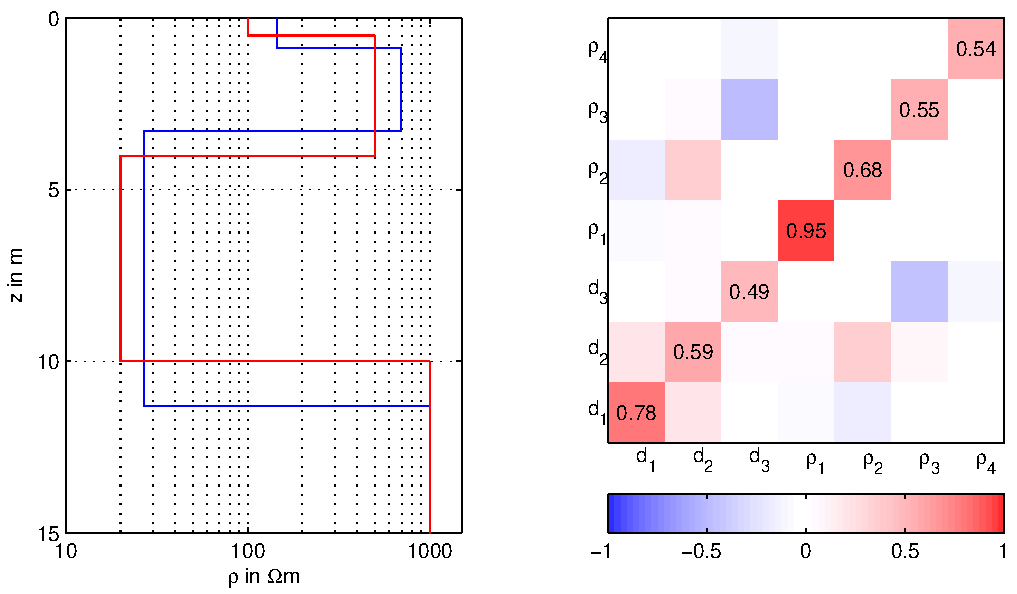
\includegraphics[width=0.7\textwidth]{dc1dblock-resres}\\[-3ex]
~\hfill a\hfill ~ \hfill ~~~~~b \hfill ~ \hfill ~ \hfill ~
\caption{a) Block 1d resistivity inversion result (red-synthetic model, blue-estimated model)) and b) resolution matrix}\label{fig:dc1dblock-resres}
\end{figure}

%%%%%%%%%%%%%%%%%%%%%%%%%%%%%%%%%%%%%%%%%%%%%%%%%%%%%%%%%%%%%%%%%%%%%%%%%%%
\subsection{Resolution analysis}\label{sec:dc1dresolution}
One may now be interested in the resolution properties of the individual model parameters.
The resolution matrix $\R^M$ defines the projection of the real model onto the estimated model:
\begin{equation}
	\m^{est} = \R^M \m^{true} + (\I - \R^M) \m^R + \S^\dagger\D\n\quad,
\end{equation}
\citep{guentherdiss} where $\S^\dagger\D\n$ represents the generalised inverse applied to the noise.
Note that $\m^R$ changes to $\m^k$ for local regularisation schemes \citep{friedel03}.

\citet{guentherdiss} also showed that the model cell resolution (discrete point spread function) can be computed by solving an inverse sub-problem with the corresponding sensitivity distribution instead of the data misfit.
This is implemented in the inversion class by the function \lstinline|modelCellResolution( iModel )| where \lstinline|iModel| is the number of the model cell.
This approach is feasible for bigger higher-dimensional problems and avoids the computation of the whole resolution matrix.
A computation for representative model cells can thus give insight of the resolution properties of different parts of the model.

For the block model we successively compute the whole resolution matrix.
\begin{lstlisting}
    RVector resolution( nModel ); //! create single resolution vector
    RMatrix resM;                 //! create empty matrix 
    for ( size_t iModel = 0; iModel < nModel; iModel++ ) {
        resolution = inv.modelCellResolution( iModel );
        resM.push_back( resolution );  //! push back the single vector
    }
    save( resM, "resM" ); //! save resolution matrix
\end{lstlisting}

In Figure~\ref{fig:dc1dblock-resres} the model resolution matrix is shown and the diagonal elements are denoted.
The diagonal elements show that the resolution decreases with depth.
The first resistivity is resolved nearly perfect, whereas the other parameters show deviations from 1.
$\rho_2$ is positively connected with $d_2$, i.e. an increase of resistivity can be compensated by an increased resistivity.
For $\rho_3$ and $d_3$ the correlation is negative.
These are the well known H- and T-equivalences of thin resistors or conductors, respectively, and show the equivalence of possible models that are able to fit the data within noise.
%Similarly, we can obtain the resolution kernels also for smooth inversion.

%%%%%%%%%%%%%%%%%%%%%%%%%%%%%%%%%%%%%%%%%%%%%%%%%%%%%%%%%%%%%%%%%%%%%%%%%%%
\subsection{Structural information}\label{sec:dc1dstruct}
{\em Example file \file{dc1dsmooth-struct.cpp} in the directory \file{doc/tutorial/code/dc1d}.}\\
Assume we know the ground water table at 4\,m from a well.
Although we know nothing about the parameters, this structural information should be incorporated into the model.
We create a thickness vector of constant 0.5\,m. 
The first 8 model cells are located above the water table, so the 8th boundary contains the known information.
Therefore we set a marker different from zero (default) after creating the mesh
\begin{lstlisting}
    //! variant 1: set mesh (region) marker
    f.mesh()->boundary( 8 ).setMarker( 1 );
\end{lstlisting}
This causes the boundary between layer 8 and 9 being disregarded, the corresponding $w^c_8$ is zero and allows for arbitrary jumps in the otherwise smoothed model.
Figure~\ref{fig:dc1dsmooth-struct} shows the result, at 4\,m the resistivity jumps from a few hundreds down to almost 10.

\begin{figure}[htbp]
\centering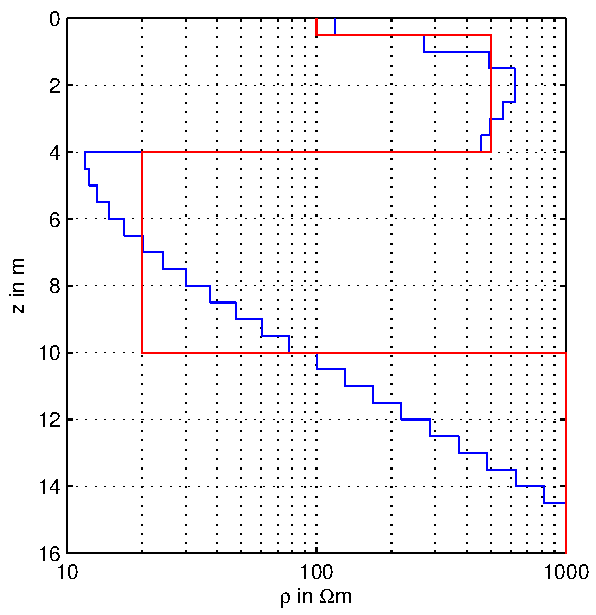
\includegraphics[width=0.45\textwidth]{sond1-100-struct.pdf}
%\\[-3ex]
%~\hfill a\hfill ~ \hfill ~~~~~b \hfill ~ \hfill ~ \hfill ~
\caption{Inversion result with the ground water table at 4\,m as structural constraint.}\label{fig:dc1dsmooth-struct}
\end{figure}

Note that we can set the weight to zero also directly, either as a property of the inversion
\begin{lstlisting}
    //! variant 2: application of a constraint weight vector to inversion
    RVector bc( inv.constraintsCount(), 1.0 );
    bc[ 6 ] = 0.0;
    inv.setCWeight( bc ); 
\end{lstlisting}
or the (only existing) region.
\begin{lstlisting}
    //! variant 3: application of a boundary control vector to region
    RVector bc( f.regionManager().constraintCount(), 1.0 );
    bc[ 7 ] = 0.0;
    f.region( 0 )->setConstraintsWeight( bc );
\end{lstlisting}
Of course, in 2d/3d inverse problems we do not set the weight by hand.
Instead, we put an additional polygon (2d) or surface (3d) with a marker $\neq 0$ into the PLC before the mesh generation.
By doing so, arbitrary boundaries can be incorporated as known boundaries.

%%%%%%%%%%%%%%%%%%%%%%%%%%%%%%%%%%%%%%%%%%
\subsection{Regions}\label{sec:dc1dregion}
{\em Example file \file{dc1dsmooth-region.cpp} in the directory \file{doc/tutorial/code/dc1d}.}\\
In the latter sections we already used regions.
A default mesh contains a region with number 0.
A block mesh contains a region 0 for the thickness values and regions counting up from 1 for the individual parameters.
Higher dimensional meshes can be created automatically by using region markers, e.g. for specifying different geological units.

In our case we can divide part above and a part below water level.
In 2d or 3d we would, similar to the constraints above, just put a region marker $\neq 0$ into the PLC and the mesh generator will automatically associate this attribute to all cells in the region.

Here we set the markers of the cells $\geq8$ to the region marker 1.
\begin{lstlisting}
    Mesh * mesh = f.mesh();
    mesh->boundary( 8 ).setMarker( 1 );
    for ( size_t i = 8; i < mesh->cellCount(); i++ ) 
        mesh->cell( i ).setMarker( 1 );
\end{lstlisting}

Now we have two regions that are decoupled automatically.
The inversion result is identical to the one in Figure~\ref{fig:dc1dsmooth-struct}.
However we can now define the properties of each region individually.
For instance, we might know the resistivities to lie between 80 and 800\,$\Omega$m above and between 10 and 100\,$\Omega$m below.
Consequently we define two transformations and apply it to the regions.
\begin{lstlisting}
    RTransLogLU transRho0( 80, 800 );
    RTransLogLU transRho1( 10, 1000 );
    f.region( 0 )->setTransModel( transRho0 );
    f.region( 1 )->setTransModel( transRho1 );
\end{lstlisting}

Additionally we might try to improve the very smooth transition between groundwater and bedrock.
We decrease the model control (strength of smoothness) in the lower region by a factor of 10.
\begin{lstlisting}
    f.region( 1 )->setModelControl( 0.1 );
\end{lstlisting}

The result is shown in Figure~\ref{fig:dc1dsmooth-region}.
The resistivity values are much better due to adding information about the valid ranges.
Furthermore the transition zone in the lower region is clear.
\begin{figure}[htbp]
\centering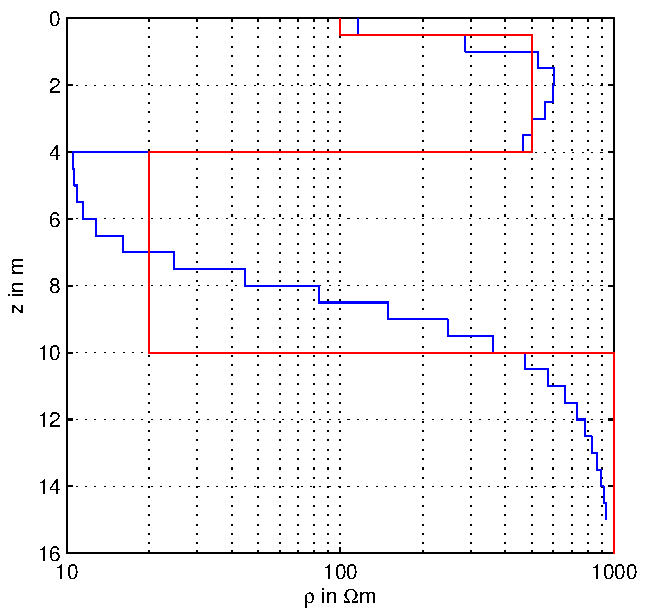
\includegraphics[width=0.45\textwidth]{sond1-100-region.pdf}
\caption{Inversion result using two regions of individual range constraint transformations and regularization strength (model control).}%
\label{fig:dc1dsmooth-region}
\end{figure}
